\documentclass[5p,authoryear]{elsarticle}
%\usepackage{paralist}
%\documentclass{article}

\begin{document}

%
% Autores
%
\title{Learning in Small and Large Ubiquitous Computing Environment}

\author[unisinos]{J.~Barbosa} 
\ead{jbarbosa@unisinos.br}

\author[unisinos]{R.~Hahn} 
\ead{rodrigo.rmh@gmail.com}

\author[unisinos]{A.~Wagner} 
\ead{andre.nho@gmail.com}

\author[unilasalle]{D.N.F.~Barbosa} 
\ead{nice@unilasalle.edu.br}

\author[ufrgs]{C.F.R.~Geyer} 
\ead{geyer@inf.ufrgs.br}

\address[unisinos]{PIPCA/Unisinos, São Leoplodo, RS, Brazil}
\address[unilasalle]{UniLasalle, Canoas, RS, Brazil} 
\address[ufrgs]{UFRGS, Porto Alegre, RS, Brazil}

%
% Abstract
%
\begin{abstract}

GlobalEdu is a generic model created to support learning in ubiquitous
computing environments. This model has the necessary support to implement
learning-related functionalities in ubiquitous environments. The basic
ubiquitous computing support must be supplied by a middleware where GlobalEdu
lays atop. This paper proposes the integration of GlobalEdu with two
middlewares: ISAM and LOCAL. ISAM supports the creation of large-scale
ubiquitous systems. As such, its integration with GlobalEdu results in
large-scale ubiquitous learning environments. On the other hand, LOCAL is
dedicated to create small-scale, location and context-aware ubiquitous
learning environments. The integration between GlobalEdu and LOCAL results in
a local ubiquitous learning system. We created a practical scenario, where our
proposal was evaluated.

\end{abstract}

\maketitle

% TODO - keywords
% TODO - agradecimentos

%
% Introduction
%
\section{Introduction}

Mobile computing \citep{weiser91} is a computational paradigm emerging from
wireless networks and distributed systems technologies. Mobility allows the
existence of various scenarios, from nomadic computing to ubiquitous computing
\citep{weiser91,satyanarayanan01}. In the last scenario, the users, carrying
portable devices (such as handhelds and notebooks) have access to a shared
infrastructure, independently from their physical location or displacement
form. In the viewpoint of ubiquitous computing, the computational power will be
available anytime and everywhere. 

In this scenario, new learning perspectives are essential, due to the
relationship between teaching and learning changes \citep{rogers05}. In our
point of view, a great amount of educational resources will soon be distributed
in a global network, and learning processes will need to explore this diversity
everywhere, anytime and in any device the learners may be employing in their
activities.  Educational applications will explore all the learning
opportunities, joining contextual information (for example, a work of art in a
museum that is being visited) with educational objectives (the learner can be
studying history of art). 

GlobalEdu is a model oriented to ubiquitous learning. It supplies the necessary
support to explore the new learning opportunities available in ubiquitous
environments. GlobalEdu is structured into layers (detailed in section 3) and
can also be coupled with an ubiquitous computing middleware (considered the
third layer). This paper proposes the integration of GlobalEdu with two
middleware projects: ISAM \citep{yamin02,augustin04} and LOCAL
\citep{barbosa07,barbosa08}. The ISAM project focuses on the building and
management of large-scale ubiquitous computing environments \citep{augustin05},
and is being developed at UFRGS (Federal University of Rio Grande do Sul,
Brazil). On the other hand, LOCAL aims to support small-scale,
location-and-context-aware computing environments. It is being developed at
UNISINOS (University of Vale do Rio dos Sinos, Brazil).

% TODO - reorganizar seções
This paper is organized as follows. Section~\ref{sec:ubisupport} presents the
definitions and standards associated with ubiquitous learning.
Section~\ref{sec:globaledu} details GlobalEdu.  Section~\ref{sec:ge-isam-local}
proposes the integration between GlobalEdu and the middleware projects ISAM and
LOCAL. Section~\ref{sec:scenario} describes a practical approach where a
small-scale scenario is being evaluated. Section~\ref{sec:related} compares our
proposal with others in the same area. Finally, Section~\ref{sec:conclusion}
presents some conclusions and plans for future work.

%
% Towards ubiquitous learning support
%
\section{Towards ubiquitous learning support} \label{sec:ubisupport}

Mobile learning (m-learning) \citep{tatar03} is fundamentally about increasing
learners' capability to carry their own learning environment along with them.
M-learning is the natural evolution of e-learning, and has the potential to
make learning even more widely accessible. However, considering the ubiquitous
view, mobile computers are still not embedded in the learners' surrounding
environment, and as such they cannot seamlessly obtain contextual information. 

An ubiquitous learning system \citep{ogata03} can use embedded devices that
communicate mutually to explore the context, and dynamically build models of
their environments. It is considered that while the learner is moving with
his/her mobile device, the system dynamically supports his/her learning by
communicating with embedded computers in the environment. The opportunities
made available by the context can be used to improve the learning experience. 

This learning scenario is attractive, but is not easily implemented. We are
investigating how to better match people's expectations for such a system. In
our point of view, ubiquitous learning environments should support the
execution of context-aware, distributed, mobile, pervasive and adaptative
learning applications. Differently from other research
projects \citep{ogata03,simon03,selene}, the GlobalEdu proposal readily
supports these characteristics. 


%
% GlobalEdu
%
\section{GlobalEdu} \label{sec:globaledu}

GlobalEdu \citep{barbosa05} aims to support ubiquitous educational
applications. Its architecture is based on a layered organization, as shown in
Figure~\ref{fig:ge-arch}. The Application Layer is represented by a
\emph{Pedagogic Agent} (PA), which follows the learner throughout the
environment and helps in her/his interactions with the system.

\begin{figure}[h!] 
  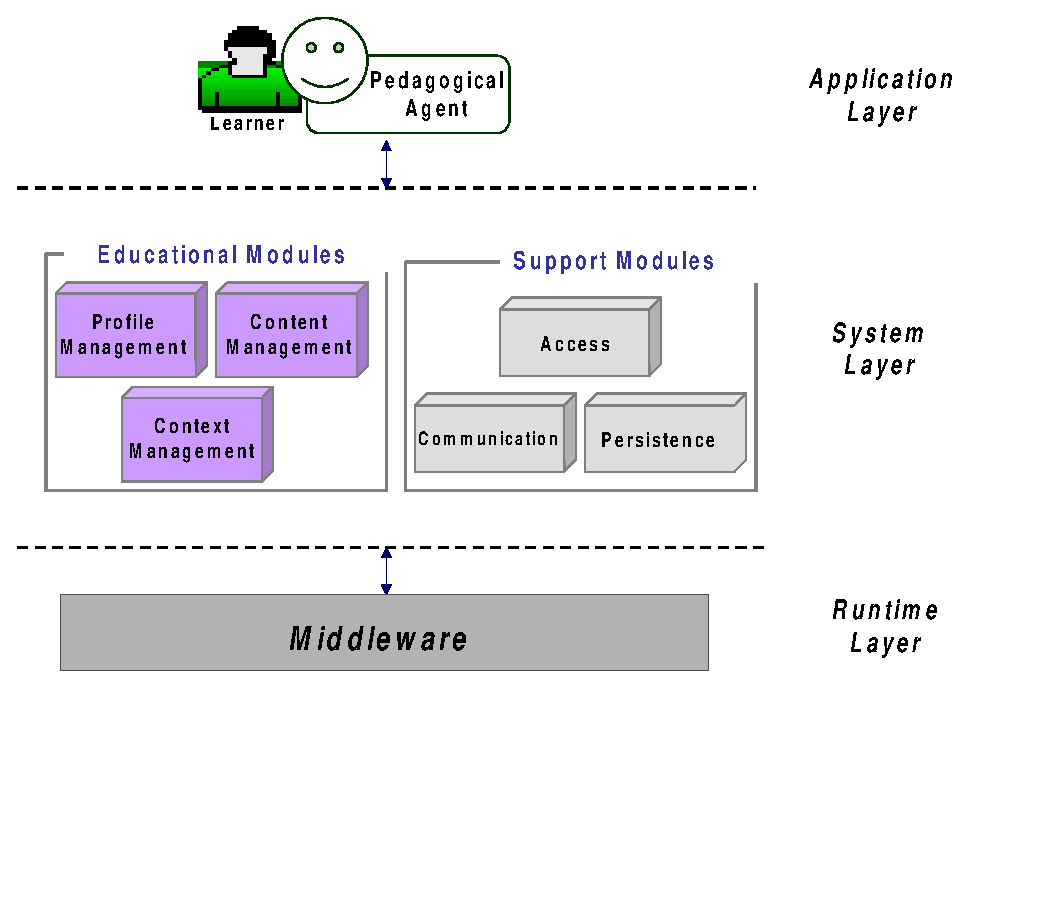
\includegraphics[width=0.5\textwidth]{media/ge-arch}
  \caption{GlobalEdu architecture} 
  \label{fig:ge-arch} 
\end{figure}
  
The \emph{System Layer} is a set of Educational Modules (EM) and Support
Modules (SM).  The Educational Modules are responsible for performing content
management tasks as well as manipulation of the learner model. The system has
three Educational Modules: Profile, Content and Context Management. The first
module is responsible for managing learner profiles. The second one deals with
the learning objects which are manipulated by the learner. The third one
controls information in the context of interest of the learner and is in charge
of adapting the resources that he/she is manipulating. The Support Modules are
intended to help in the execution of the Educational Modules and the
Pedagogical Agent, by managing the aspects of communication, adaptation of
interfaces to devices, user's access and persistence.  

The Runtime Layer is a middleware which supports the execution of educational
applications, providing the system with necessary features, such as perception
of contextual elements, code migration and communication mechanisms.  

For us, one of the characteristics of ubiquitous learning is that the user's
context can be connected with the learner's local context, joining this
information with educational objectives. The \emph{Context Management} module
manages learner context in each location the learner interacts. This module
detects changes of contextual elements in the different locations where the
learner is.  The \emph{Social Context} and \emph{Physical Context} compose the
learner context.  

The \emph{Social Context} has contextualized information about Location Context
and the presence of other PAs in the current context. Location Context contains
information about People (name, e-mail, commitments and roles), Events (type,
description and location) and Resources (name, type, description and
commitments) related to a specific location. The presence of other PAs
presupposes the existence of other learners with the same goals, competencies
and preferences, whose information the learner may access for contact or not.
This information can also be used for the creation of learner groups within the
same context.  

The \emph{Physical Context} represents the resources accessed by the learner,
such as network, locations and devices. We consider that the ubiquitous
computing environment monitors Physical Context elements. Besides, any element
state changes are informed to the \emph{Context Management}.

The \emph{Context Management} module has the capability to know how to locate
the learner in his/her current environment, to identify a learner in the
corresponding context and to provide information adapted to the device the
learner is using. In the same way, each location is modeled as a Geographic
Region and has information about Location Context. So, for GlobalEdu, the
ubiquitous environment is composed by cells and these have different contexts
(Figure~\ref{fig:ge-env}). For example, a University can be considered a cell
and its buildings, different contexts. 

\begin{figure}[h!] 
  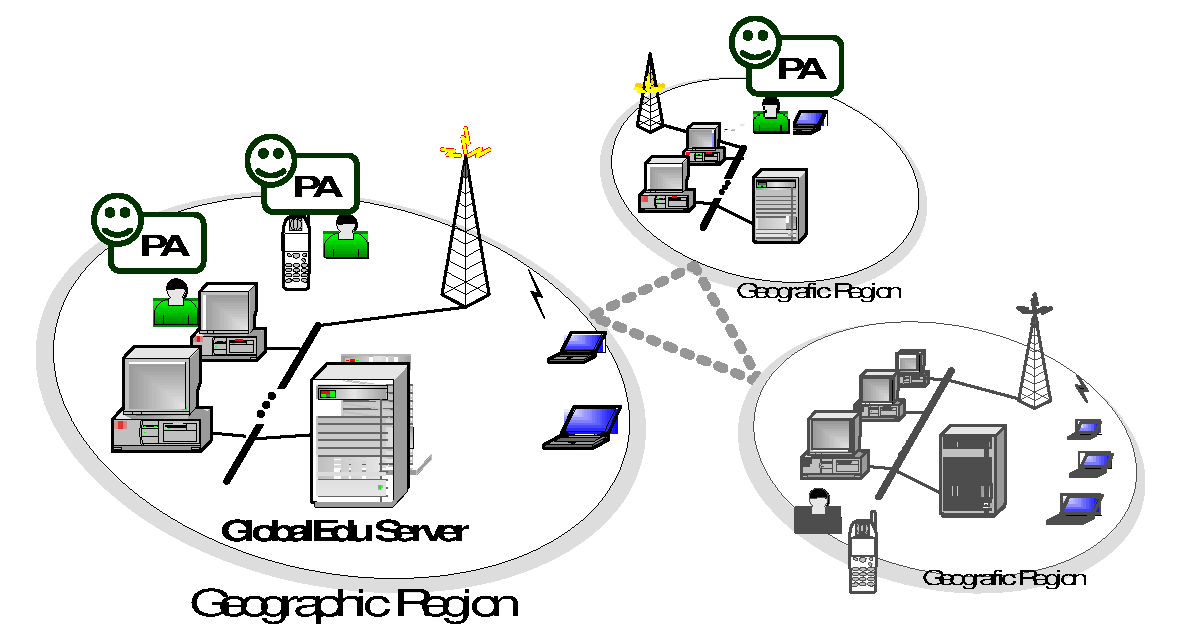
\includegraphics[width=0.5\textwidth]{media/ge-env}
  \caption{The GlobalEdu environment} 
  \label{fig:ge-env}
\end{figure}
  
Learners need to authenticate themselves in order to interact with the
environment. This event is handled by the \emph{Context Management} module.
When a new learner enters into the environment, the Social Context changes. In
this case, the service takes two actions: (1)~notifies other learners in the
corresponding context (Location Context), and (2)~sends to the new learner
adapted information about the current context he/she is in. User profiles are
compared in order to define learners with the same goals, competencies and
preferences, whose information the learner may access for contact or not.  

For the adaptation process, there is a relationship between the \emph{Context
Management} module and the other elements of the architecture (see
Figure~\ref{fig:context-mgmt}). 
  
\begin{figure}[h!] 
  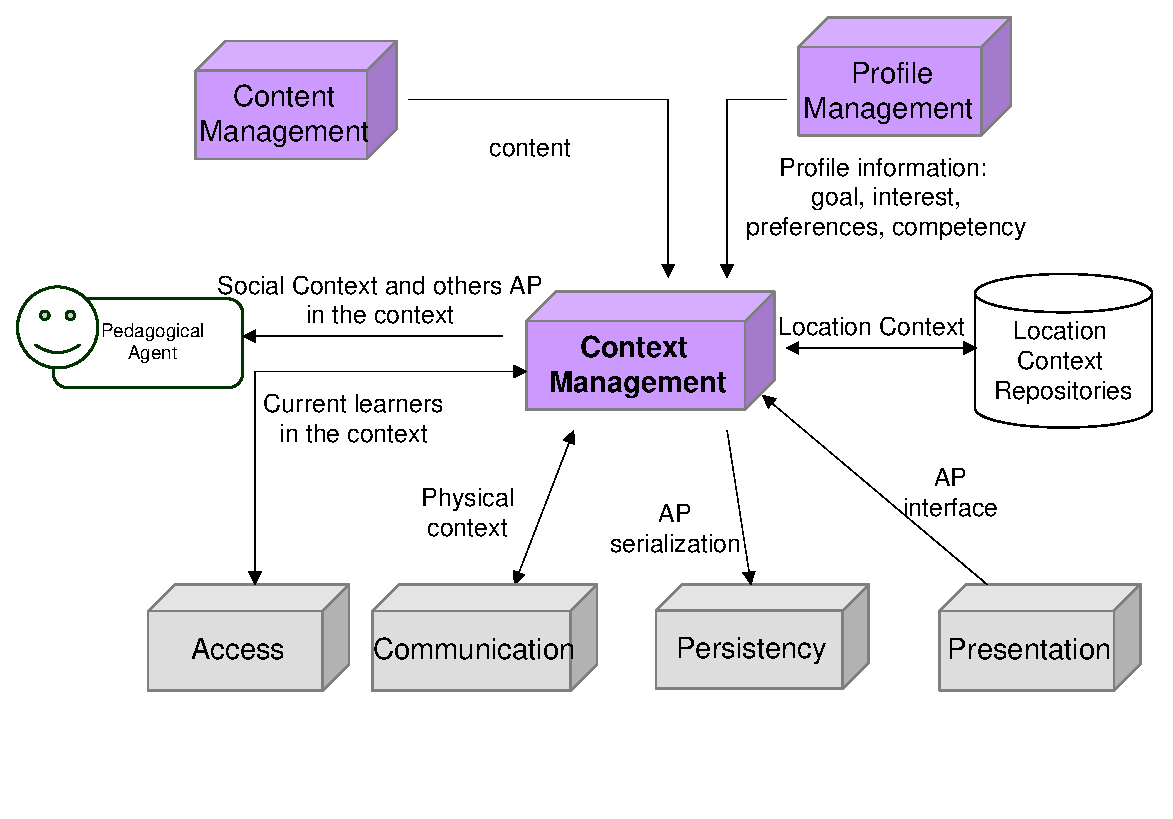
\includegraphics[width=0.5\textwidth]{media/context-mgmt}
  \caption{Context management} 
  \label{fig:context-mgmt} 
\end{figure}
  
With this, learners can ask explicit information about the Social Context they
are part of. He can also extend the search for information to other contexts.
This can be useful in the case of finding learning objects related to the
learner's goals, for instance. 

%
% GlobalEdu, ISAM and LOCAL
%
\section{GlobalEdu, ISAM and LOCAL} \label{sec:ge-isam-local}

GlobalEdu is a generic model created in order to support ubiquitous learning.
This model supports the basic features needed to implement learning-related
functionalities in ubiquitous environments. The basic ubiquitous computing
support must be supplied by a middleware (see Figure~\ref{fig:ge-arch}).
GlobalEdu has been integrated with two ubiquitous environments: ISAM
\citep{yamin02,augustin04} and LOCAL \citep{barbosa07,barbosa08}. ISAM supports
the creation of large-scale ubiquitous systems. As such, its integration with
GlobalEdu results in a large-scale ubiquitous learning system.  On other hand,
LOCAL is dedicated to create small-scale location and context-aware ubiquitous
systems. GlobalEdu integrated with LOCAL results in a local ubiquitous learning
system. 


%
% Large-scale: GlobalEdu and ISAM
%
\subsection{Large-scale: GlobalEdu and ISAM} \label{sec:ge-isam}

The ISAM Project \citep{yamin02,augustin04} provides a common system platform,
allowing the execution of applications across a wide range of equipment as well
as automatic distribution and installation. ISAM is based on the vision that
ubiquitous applications are distributed, mobile and context-aware by nature,
and assumes that ``the computer'' is the whole network (large-scale
pervasiveness). The ISAM Pervasive Environment (ISAM\emph{pe}) is composed of
elements that correspond to the physical infrastructure of the mobile network.
The physical organization adopted in ISAM is the cellular hierarchy (see
Figure~\ref{fig:ge-isam}). Each cell has a base and the cells are connected to
support the ubiquitous environment. A cell manages nodes such as desktops and
mobile devices which can be connected either by wired or wireless networks.

\begin{figure}[h!] 
  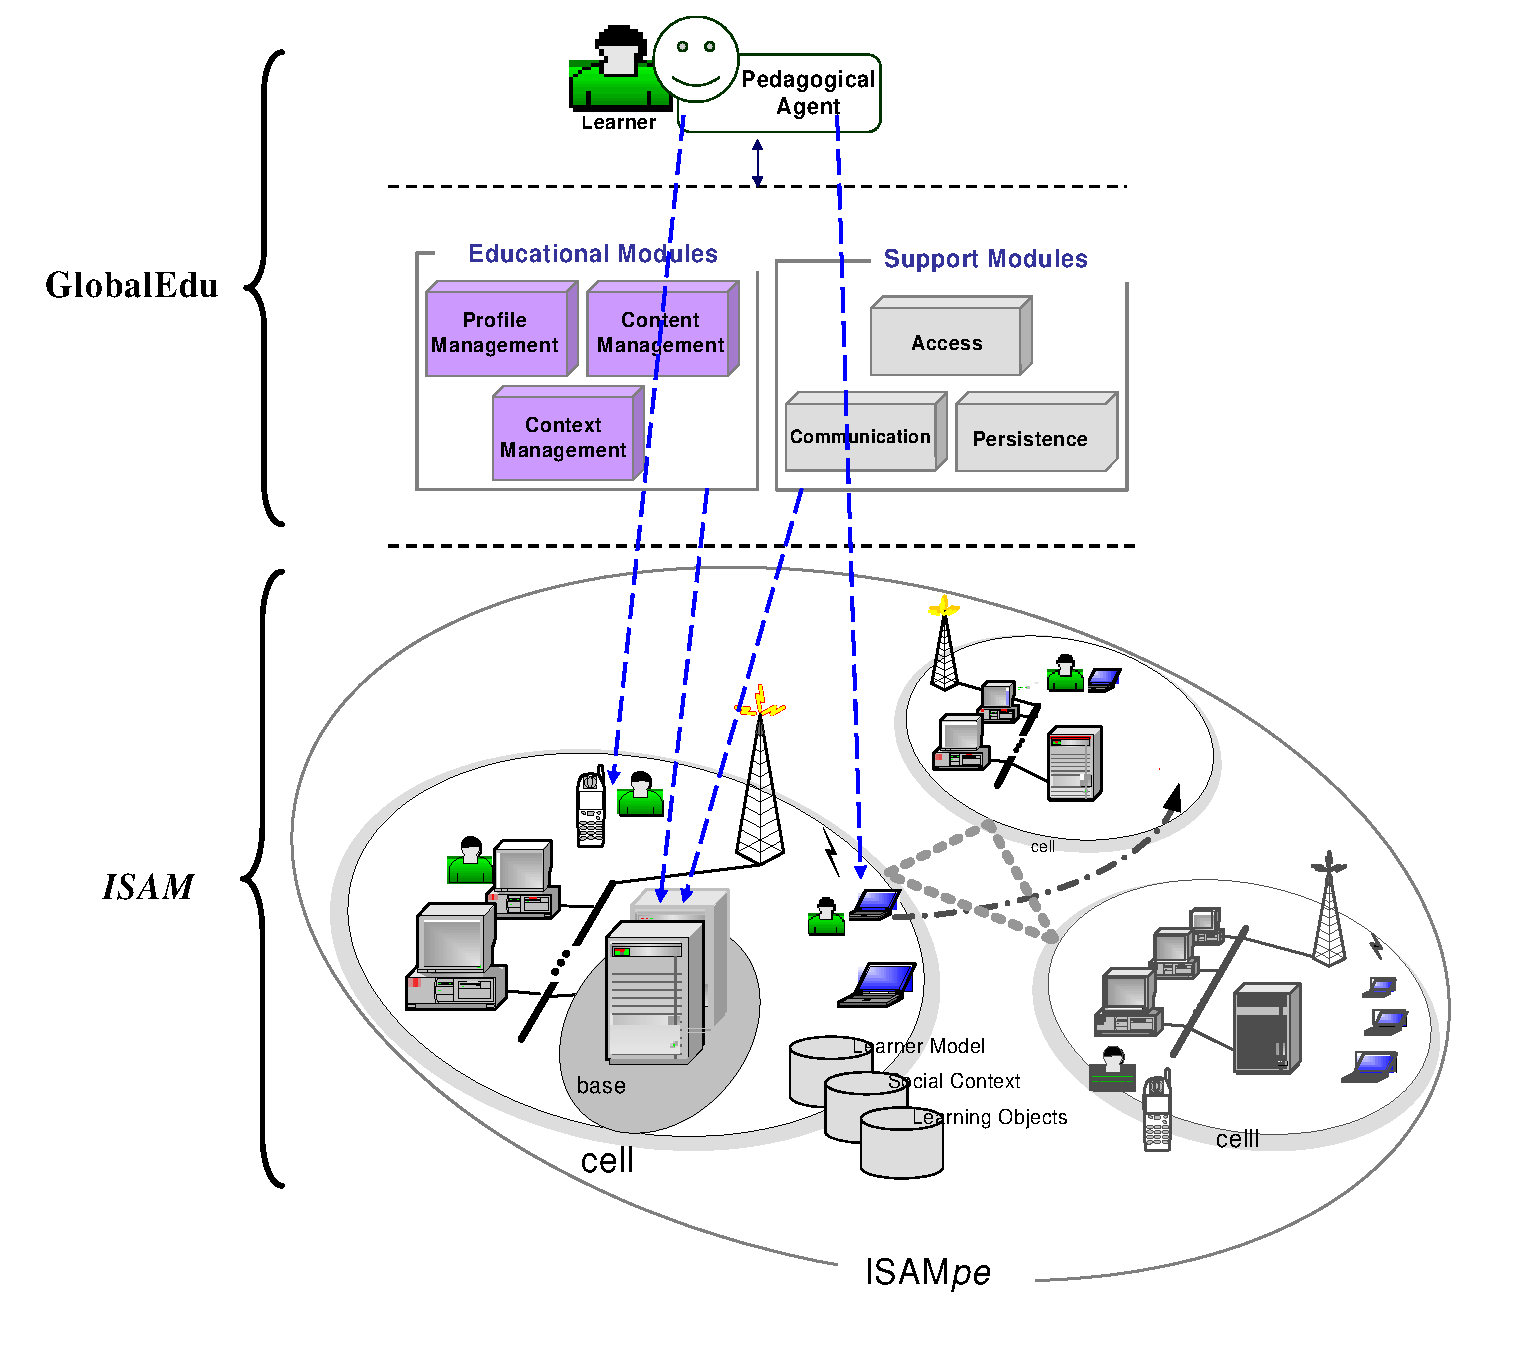
\includegraphics[width=0.5\textwidth]{media/ge-isam}
  \caption{GlobalEdu and ISAM} 
  \label{fig:ge-isam} 
\end{figure}

As can be seen in the Figure~\ref{fig:ge-env}, GlobalEdu also uses a cellular
hierarchy. It is possible to map the GlobalEdu architecture to ISAM (as shown
in Figure~\ref{fig:ge-isam}). The Pedagogical Agent (PA) is mapped to mobile
nodes and the Educational and Support Modules are mapped to the bases (servers
in a cell). The Modules are heavyweight execution units, and are executed in
network servers. On the other hand, PA is a lightweight execution unit, so it
can be executed in mobile devices.

Each ISAM cell has one instance of GlobalEdu. Users can change their context
(cell), carrying their PA. ISAM supports the basic ubiquitous computing-related
aspects and GlobalEdu supports the specific learning aspects.   

%
% Small-scale: GlobalEdu and LOCAL
%
\subsection{Small-scale: GlobalEdu and LOCAL} \label{sec:ge-local}

The LOCAL project \citep{barbosa07,barbosa08} aims to provide a
location-and-context-aware ubiquitous architecture geared to create small-scale
learning environments.  LOCAL is composed by seven subsystems (see
Figure~\ref{fig:local-arch}): (1)~\emph{User Profiles}, which store information
related to the users using the PAPI standard [14]; (2)~\emph{Personal
Assistant}, which acts as the system's interface, residing in the user's mobile
device; (3)~\emph{Location System}, used to determine the physical position of
the mobile devices; (4)~\emph{Learning Objects Repository}, which stores and
indexes content related to the teaching process; (5)~\emph{Tutor}, an analysis
engine capable of making inferences by using the data supplied by the profiles
and the location system; (6)~\emph{Communication System}, used to establish
communication between the different parts of LOCAL, and between the system and
its users; (7)~\emph{Event System}, used to schedule tasks. 

\begin{figure}[h!] 
  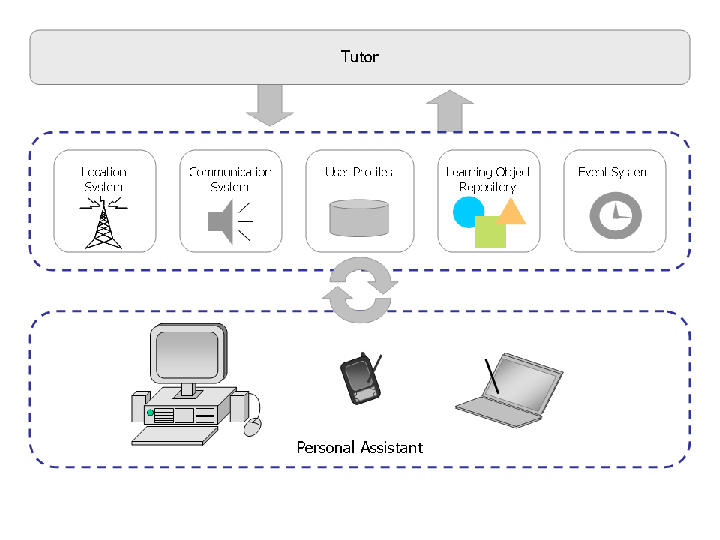
\includegraphics[width=0.5\textwidth]{media/local-arch}
  \caption{The LOCAL architecture} 
  \label{fig:local-arch} 
\end{figure}
  
The \emph{personal assistant} (PA) is the module which accompanies the learner
in its mobile device. It allows users to stay connected to the system, while
providing a certain degree of independence. The \emph{location system} ties
users' physical location data to symbolic names (contexts). This allows real
time mapping of mobile device positions.  As the learner authorizes the
location system in its PA, it begins to determine the device's position and
physical context changes, along with the time and date of such changes. With
this data, it is possible to completely track the learner's movements. User
profile data, alongside context information, is used in the learning process.
  
\emph{Learning objects} in LOCAL are made available to learners in accordance
with whatever pedagogical opportunities may appear during their interaction
with the different contexts. The location system keeps the tutor aware of which
context the learner is in. The tutor uses this information, as well as the
learner's profile data, to select the objects meeting the learner's goals and
the context. The objects meeting these criteria are then forwarded to the
learner.  The metadata specification for Learning Objects in LOCAL was made in
accordance with the IEEE LTSC \citep{ieee08a}. The \emph{tutor} uses profile
and location data to find learning opportunities. It can act in two ways:
(1)~providing relevant, contextualized learning objects and (2)~stimulating
interaction between learners, by using learner profile data to create bonds
between learners.
  
GlobalEdu uses the services offered by LOCAL to monitor and control the
environment (see Figure~\ref{fig:local-ge}). GlobalEdu´s PAs are executed in
the learner's devices, mapped to the LOCAL Personal Assistant. The Location
System and the Event System are used to support the Context Management Module.
Context Management Module is supported by the Learning Object Repository and
the Profile Management by the User Profiles System. Communication Support
Module is mapped to the LOCAL Communication System. Other Support Modules are
not used. 
  
LOCAL is oriented to small-scale ubiquitous environments and its architecture
was projected to a centralized execution (only one server). As such, there is
only one GlobalEdu instance (see Figure~\ref{fig:ge-arch}). Modules are
executed in the network server and the PA executes in the users' mobile
devices.


\section{Practical scenario: GlobalEdu and LOCAL} \label{sec:scenario}


\section{Related work} \label{sec:related}


\section{Conclusion} \label{sec:conclusion}

%
% Bibliografia
%
\bibliographystyle{plainnat} \bibliography{globaledu_local}


\end{document}
